\documentclass{standalone}
\usepackage{xcolor}

\usepackage{caslondeco}
\usepackage{marvosym}
\usepackage{fontawesome}

\begin{document}
\begin{tikzpicture}[x=12pt, y=12pt]

  % Define dimensions
  \def\cardWidth{3.5in}
  \def\cardHeight{2.0in}
  \def\margin{11pt}
  \def\strokeWidth{8pt}

  %% draw an invisible border so the page crops to this instead of content
  \draw[black!20, line width=1pt] (0,0) rectangle (\cardWidth,\cardHeight);
  \clip (0,0) rectangle (\cardWidth,\cardHeight);

  \drawxgrid{%
    Nx=21,%
    Ny=12,%
    displaywidth=3.5in,
    displayheight=2in,
    color=black!40!white,
    yshift=0.5,
    flrmodval=4,
    xshift=1.0, 
    initial={\footnotesize \textsw{A}}
  }

  \filldraw[
    fill=black!2!white,
    draw=black,
    style=double,
    double distance=2pt,
    line width=0.8pt
  ]
  (0.15*\cardWidth,\cardHeight/2)
  -- (0.5*\cardWidth,0.9*\cardHeight)
  -- (0.85*\cardWidth,\cardHeight/2)
  -- (0.5*\cardWidth,0.1*\cardHeight)
  -- cycle;

  \node[draw=none, align=center, yshift=-3pt] at (\cardWidth/2, \cardHeight/2) (ctr) {
    \Telefon \;\; (123) 456-789 \\
    \Letter \;\; 5 Wallowing Dove Ln \\
    \faBriefcase \;\; \textit{Chief Good Times Officer} \\
    \Industry \;\; Ministry of Recreation \\
    \Football \;\; Thursdays @ 5pm \\
    \Lightning
  }; 

\end{tikzpicture}
\end{document}
